%% RadAlert-AT: Cross-Study Radiation-Exposure Triage from Plant Gene Expression
%% ACDSA 2027 two-column manuscript (IEEE conference template).
\documentclass[10pt,conference]{IEEEtran}
\usepackage{paperstyle}

\graphicspath{{figures/}}

\begin{document}

\title{Reframing Plant Radiation Dosimetry as Cross-Study Exposure Triage}

\author{
\IEEEauthorblockN{Sanvi Desai\equalcontrib}
\IEEEauthorblockA{Nexus Labs\\ Palo Alto, USA\\ sanvidesai17@gmail.com}
\and
\IEEEauthorblockN{Sushant Donadi\equalcontribmark}
\IEEEauthorblockA{Nexus Labs\\ Palo Alto, USA\\ sushantdonadi@gmail.com}
\and
\IEEEauthorblockN{Gayatri Goli\equalcontribmark}
\IEEEauthorblockA{Nexus Labs\\ Palo Alto, USA\\ gayatri.shannu@gmail.com}
\and
\IEEEauthorblockN{Soham Gupta\equalcontribmark}
\IEEEauthorblockA{Nexus Labs\\ Palo Alto, USA\\ sohamgupta12@gmail.com}
\and
\IEEEauthorblockN{Aswath Madhan\equalcontribmark}
\IEEEauthorblockA{Nexus Labs\\ Palo Alto, USA\\ aswathmadhan09@gmail.com}
\and
\IEEEauthorblockN{Jackson Szekeres\equalcontribmark}
\IEEEauthorblockA{Nexus Labs\\ Palo Alto, USA\\ jdszekeres@gmail.com}
\and
\IEEEauthorblockN{Srikanth Samy}
\IEEEauthorblockA{University of California, Berkeley\\ Berkeley, USA\\ ssamy@berkeley.edu}
\and
\IEEEauthorblockN{Ishaan Gupta}
\IEEEauthorblockA{Stanford University\\ Stanford, USA\\ ishaangupta@stanford.edu}
}

\maketitle

\begin{abstract}
Predicting absorbed radiation dose from gene expression is an attractive framing, but it
is only answerable if the underlying experiments actually span the dose axis. Auditing a
six-study collection of \emph{Arabidopsis thaliana} RNA-seq profiles ($158$ samples,
$4{,}002$ genes, NASA OSDR), we find that $138$ of $158$ samples sit at exactly $0$ or
$100$~Gy and only $20$ represent intermediate doses---a design that supports
exposed-versus-control triage but not a calibration curve. We therefore change the
target and report both outcomes. Under leave-one-study-out validation, in which an
entire study is withheld and all adaptive operations including gene selection are fitted
inside the training folds, a $50/100$-gene stability ensemble reaches $84.2\%$ pooled
accuracy, $82.4\%$ balanced accuracy, $0.883$ pooled ROC-AUC, $0.656$ Matthews
correlation, $89.0\%$ sensitivity, and $75.9\%$ specificity. The same protocol applied to
exact-dose regression yields $33.6$~Gy mean absolute error and Spearman $\rho=0.523$: the
negative result that motivated the reframing. Because the independent unit is a study
and not a sample, we bootstrap over the six study-level scores rather than over the $158$
samples, giving a macro balanced accuracy of $0.849$ with a $95\%$ interval of
$[0.757,0.938]$---broad, and honestly so. Three canonical DNA-damage-response genes are
selected in every outer fold, which makes the classifier biologically plausible without
establishing that its markers are specific to radiation rather than to stress in general.
\end{abstract}

\paperkeywords{Arabidopsis, domain generalization, gene expression, leave-one-study-out
validation, radiation biology, study design, triage}

\section{Introduction}
A predictive question is only as good as the experimental design behind it. Asking a
model to estimate absorbed radiation dose from a transcriptome presupposes that the
available data samples the dose axis densely enough for a dose--response relationship to
be identifiable. When it does not, a regression can still be fitted, a correlation can
still be reported, and the resulting number can look like partial success while in fact
measuring something closer to group separation.

This paper is a worked example of catching that failure and responding to it. Working
with six NASA Open Science Data Repository studies of irradiated \emph{Arabidopsis
thaliana}~\cite{osdr}, we audit the target before modelling it, find that the dose axis
is effectively binary, and reframe the task as the operational question the data can
support: \emph{given an expression profile from a study never seen during training, was
this plant irradiated?}

\subsection{Contributions}
\begin{enumerate}
\item A target-design audit that rejects the originally posed regression on
      identifiability grounds, with the failed regression retained and reported rather
      than discarded.
\item A leakage-controlled cross-study benchmark in which the held-out unit is an entire
      study and all feature selection, scaling, and fitting occur inside the training
      folds, comparing a literature panel against linear, kernel, tree, and ensemble
      models.
\item Uncertainty quantified at the correct level of analysis. With six independent
      studies, we bootstrap study-level scores rather than samples, which widens the
      intervals substantially and reflects what the design actually supports.
\item A stability analysis of repeatedly selected genes, with an explicit statement of
      why concordance with the DNA-damage-response literature is plausibility evidence
      and not biomarker validation.
\end{enumerate}

\section{Data and Design Audit}

\subsection{Cohort}
The harmonized matrix contains $158$ samples $\times$ $4{,}002$ genes drawn from six
studies (OSD-498, 502, 508, 510, 658, 782), with a manifest recording absorbed dose,
radiation quality (gamma or heavy ion), genotype, and tissue. Of the $158$ samples,
$58$ are unirradiated controls and $100$ are exposed.

\subsection{Why exact dose is not identifiable here}
\cref{fig:audit}(a) shows the distribution of absorbed dose. Four of the six studies
contain only $0$ and $100$~Gy. Pooling everything, $138$ of $158$ samples ($87\%$) sit at
one of those two extremes; $10$, $40$, and $80$~Gy together contribute $20$ samples,
with only four samples at each of $40$ and $80$~Gy.

A regression trained on this support cannot distinguish a genuine dose--response gradient
from a two-group contrast. Reporting Spearman $\rho\approx0.52$ for such a model is
technically correct and substantively misleading: with $87\%$ of the mass at two points,
a rank correlation is dominated by the model's ability to separate those two points, not
by any calibration in between. We therefore change the endpoint to
\begin{equation}
y_i=\ind\!\left[\text{dose}_i>0\ \text{Gy}\right],
\label{eq:target}
\end{equation}
and revisit the regression in \cref{sec:regression} as a reported negative result.

\begin{figure*}[!t]
\centering
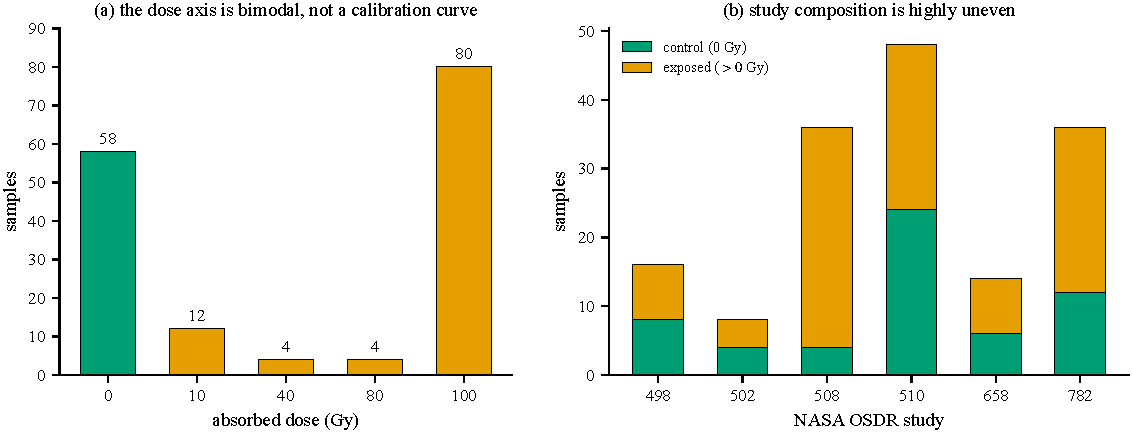
\includegraphics[width=\textwidth]{fig1_design_audit.pdf}
\caption{(a) The absorbed-dose distribution is bimodal: $138$ of $158$ samples lie at
$0$ or $100$~Gy, and the intermediate levels carry $12$, $4$, and $4$ samples
respectively. (b) Study composition is highly uneven; OSD-508 is $88.9\%$ exposed while
OSD-510 is balanced, so any protocol that ignores study membership will confound
exposure with batch.}
\label{fig:audit}
\end{figure*}

\subsection{Preprocessing provenance}
The distributed matrix is log-transformed, per-study standardized, and restricted to the
$4{,}002$ most variable genes. Per-study standardization suppresses laboratory-scale
batch effects~\cite{leek2010batch}, but it is transductive: it uses the distribution of
an entire study, including its test samples, before any label is predicted. Our benchmark
is therefore conditional on this supplied representation. A deployable pipeline would
require a reference-based normalization that can transform a single incoming sample, and
we flag this as the principal gap between the present result and a usable assay.

\section{Evaluation Protocol}

\subsection{Leave-one-study-out}
Randomly splitting samples would place the same laboratory, genotype, growth protocol,
and sequencing batch on both sides of the split, estimating interpolation within known
studies rather than transfer to a new one~\cite{steyerberg2016}. We instead hold out one
complete study at a time:
\begin{equation}
\hat{p}^{(s)} = f_{\mathcal{D}\setminus s}\!\left(\mathbf{x}\right),
\qquad \mathbf{x}\in s,\quad s\in\mathcal{S},\ |\mathcal{S}|=6 .
\label{eq:loso}
\end{equation}
Every adaptive operation---the ANOVA $F$-test gene selector, the scaler, and the
classifier---is refitted on $\mathcal{D}\setminus s$ alone. Selecting genes on the full
matrix before cross-validation is the classic inflation mechanism in expression
studies~\cite{ambroise2002}, and \cref{eq:loso} is specified precisely to exclude it.
The decision threshold is fixed at $0.5$ throughout and is never tuned.

\subsection{Metrics}
Because $63.3\%$ of samples are exposed, accuracy alone is inadequate: the trivial
always-exposed rule scores $0.633$. We therefore report balanced accuracy,
ROC-AUC~\cite{fawcett2006}, average precision, sensitivity, specificity, and the
Matthews correlation coefficient
\begin{equation}
\mathrm{MCC}=\frac{\mathrm{TP}\cdot\mathrm{TN}-\mathrm{FP}\cdot\mathrm{FN}}
{\sqrt{(\mathrm{TP}{+}\mathrm{FP})(\mathrm{TP}{+}\mathrm{FN})(\mathrm{TN}{+}\mathrm{FP})(\mathrm{TN}{+}\mathrm{FN})}},
\label{eq:mcc}
\end{equation}
which uses all four confusion-matrix cells and is the appropriate single summary under
class imbalance~\cite{chicco2020}.

\subsection{Model ladder}
Five models plus a baseline are compared, in increasing flexibility: (i) the
always-exposed rule; (ii) DDR-7, logistic regression on seven literature
DNA-damage-response genes; (iii) top-50 logistic regression with fold-local selection;
(iv) a top-100 RBF-SVM; (v) top-100 extremely randomized trees~\cite{geurts2006}; and
(vi) a stability ensemble averaging tree probabilities from the top-50 and top-100
training-fold panels. The ensemble is motivated by stability
selection~\cite{meinshausen2010}: averaging over two panel sizes removes the arbitrary
choice of a single $k$.

\section{Results}

\subsection{Cross-study benchmark}
\cref{tab:models} and \cref{fig:ladder} give the leave-one-study-out results.

\begin{table*}[!t]
\centering
\caption{Leave-one-study-out performance, six folds, threshold fixed at $0.5$. All
adaptive operations are fitted inside the training studies.}
\label{tab:models}
\begin{tabular}{lrrrrrr}
\toprule
Model & Acc. & Bal.\ acc. & ROC-AUC & MCC & Sens. & Spec.\\
\midrule
Stability ensemble  & \textbf{0.842} & \textbf{0.824} & 0.883 & \textbf{0.656} & 0.890 & 0.759\\
Top-100 ExtraTrees  & 0.823 & 0.806 & \textbf{0.886} & 0.616 & 0.870 & 0.741\\
Top-50 logistic     & 0.791 & 0.799 & 0.859 & 0.579 & 0.770 & \textbf{0.828}\\
Top-100 RBF-SVM     & 0.804 & 0.783 & 0.878 & 0.574 & 0.860 & 0.707\\
DDR-7 logistic      & 0.741 & 0.770 & 0.741 & 0.521 & 0.660 & 0.879\\
Always exposed      & 0.633 & 0.500 & 0.500 & 0.000 & 1.000 & 0.000\\
\bottomrule
\end{tabular}
\end{table*}

\begin{figure*}[!t]
\centering
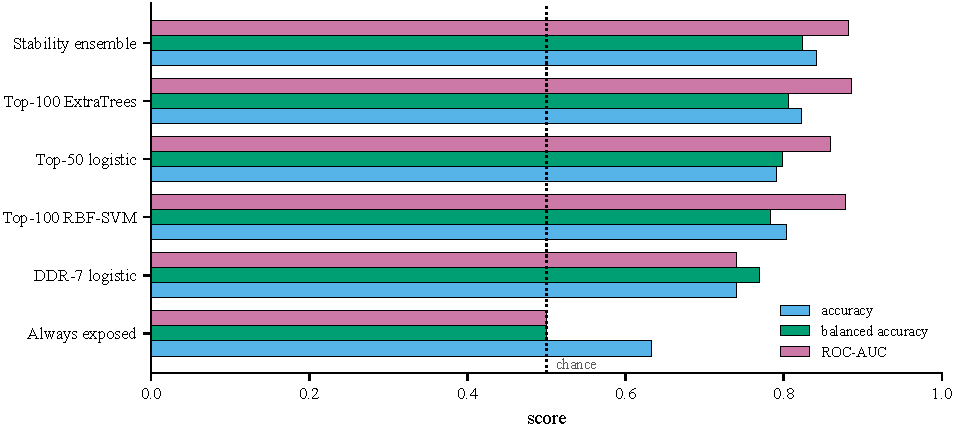
\includegraphics[width=0.86\textwidth]{fig2_model_ladder.pdf}
\caption{The model ladder. The always-exposed rule attains $0.633$ accuracy with $0.500$
balanced accuracy and zero specificity, which is exactly why accuracy is not the primary
endpoint. Fold-local multigene models improve substantially on the literature panel.}
\label{fig:ladder}
\end{figure*}

Three comparisons matter. First, the always-exposed rule makes the case for balanced
metrics concrete: $0.633$ accuracy, $0.500$ balanced accuracy, zero specificity. Second,
the seven-gene literature panel is genuinely informative ($\mathrm{MCC}=0.521$) and has
the second-highest specificity in the table, but its ROC-AUC of $0.741$ is well below
every fold-local multigene model---the canonical DDR genes carry real signal but not all
of it. Third, the stability ensemble gives the best thresholded performance
($\mathrm{MCC}=0.656$), though its pooled AUC ($0.883$) is statistically
indistinguishable from the single top-100 tree model ($0.886$). The ensemble's advantage
is in calibration at the fixed threshold, not in ranking.

\subsection{Error structure}
\cref{fig:errors} decomposes the ensemble's errors. The pooled confusion matrix is
$\mathrm{TP}=89$, $\mathrm{FN}=11$, $\mathrm{TN}=44$, $\mathrm{FP}=14$: sensitivity
$89.0\%$ against specificity $75.9\%$. The asymmetry is consistent throughout the model
ladder and is the operationally important weakness---roughly one unirradiated control in
four is flagged as exposed, which for a screening instrument means the positive calls
require confirmation.

\begin{figure*}[!t]
\centering
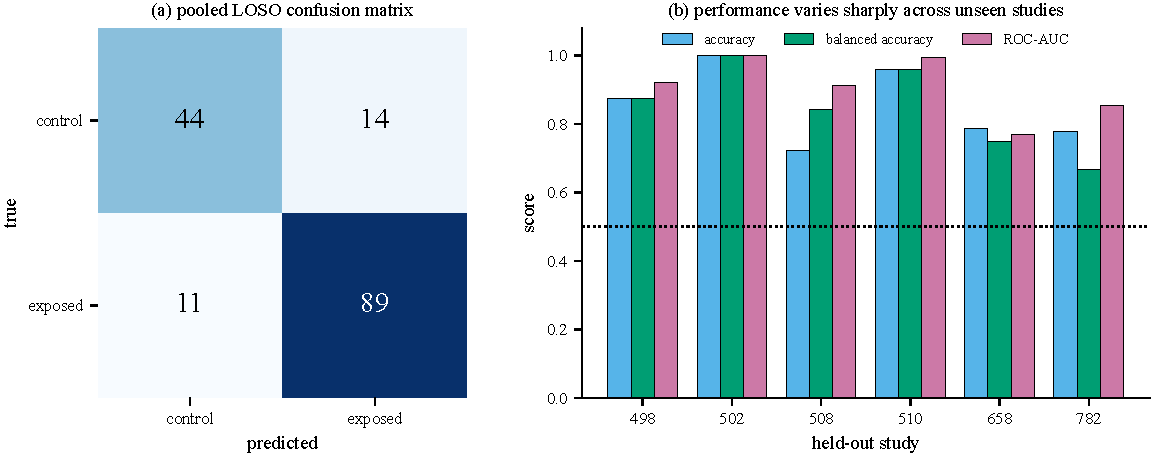
\includegraphics[width=\textwidth]{fig3_error_analysis.pdf}
\caption{(a) Pooled confusion matrix for the stability ensemble. Specificity ($75.9\%$)
lags sensitivity ($89.0\%$). (b) Per-study performance. OSD-502 is perfectly classified
and OSD-510 nearly so, while OSD-782 falls to $66.7\%$ balanced accuracy despite an AUC
of $0.854$---a threshold problem, not a ranking failure.}
\label{fig:errors}
\end{figure*}

Per-study performance ranges widely: OSD-502 is perfectly separated
($\mathrm{AUC}=1.000$, $n=8$), OSD-510 nearly so ($0.993$, $n=48$), while OSD-658 falls
to $0.771$ and OSD-782 to $0.667$ balanced accuracy. OSD-782's case is diagnostic. Its
AUC is a respectable $0.854$, so the ranking is sound; what fails is the fixed $0.5$
threshold on that study's score distribution. A held-out study can therefore be
well-ordered and still be badly classified, which is an argument for reporting both a
ranking and a thresholded metric rather than either alone.

\subsection{Do intermediate doses register?}
The intermediate levels are far too sparse for dose--response claims, but they test
whether the binary model merely memorised the $100$~Gy condition.
\cref{fig:dose}(a) shows the mean held-out exposure score rising with dose and remaining
above the threshold at $10$, $40$, and $80$~Gy. With $n=12$, $4$, and $4$ respectively,
these points are descriptive only; the correct reading is that the classifier is not
purely a $100$~Gy detector, not that it is calibrated across dose.

\begin{figure*}[!t]
\centering
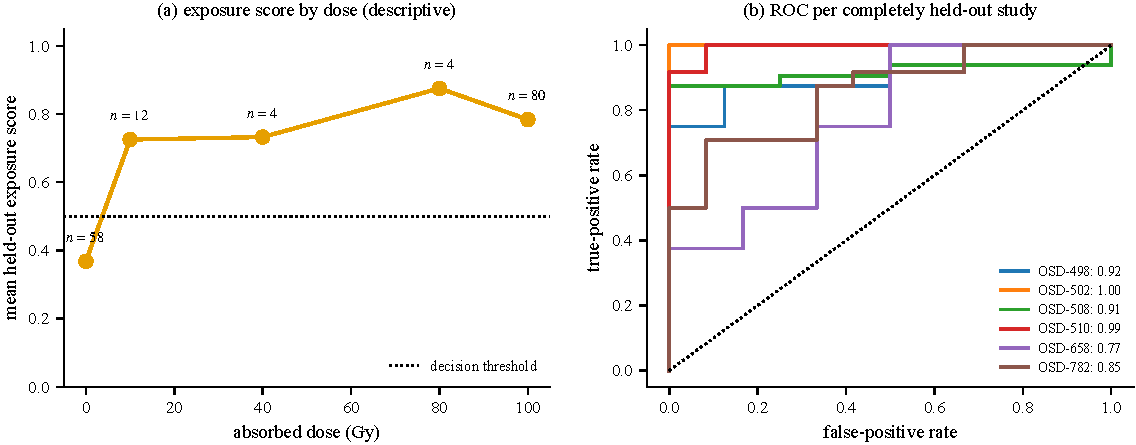
\includegraphics[width=\textwidth]{fig4_dose_and_roc.pdf}
\caption{(a) Mean held-out exposure score by dose. Intermediate doses score above the
threshold, but with $n\le12$ per level these are descriptive points, not population
estimates. (b) ROC curves for each completely held-out study, showing the spread that a
pooled curve conceals.}
\label{fig:dose}
\end{figure*}

\subsection{Uncertainty at the right unit of analysis}
There are $158$ samples but only six independent external validation studies. Samples
within a study share genotype, growth conditions, harvest, and sequencing batch, so
treating them as independent replicates would produce intervals that are far too narrow
for the design~\cite{varoquaux2018}. We therefore bootstrap the six study-level
scores~\cite{efron1986}. \cref{tab:uncertainty} reports the result.

\begin{table*}[!t]
\centering
\caption{Study-level bootstrap, $B=10{,}000$ resamples of the six held-out studies. The
intervals are broad because the design supports six independent observations, not $158$.}
\label{tab:uncertainty}
\begin{tabular}{lrr}
\toprule
Macro-averaged metric & Estimate & $95\%$ interval\\
\midrule
Accuracy          & 0.853 & $[0.777,\ 0.937]$\\
Balanced accuracy & 0.849 & $[0.757,\ 0.938]$\\
ROC-AUC           & 0.909 & $[0.846,\ 0.970]$\\
\bottomrule
\end{tabular}
\end{table*}

The macro balanced-accuracy interval spans $18$ percentage points. That width is the
honest headline of this study: the point estimate is encouraging, and the design cannot
presently distinguish $0.76$ from $0.94$.

\subsection{Which genes are selected consistently?}
Repeating the fold-local selector and counting how often each gene enters the top-100
panel gives a stability profile that, unlike a single fit, cannot be driven by one
study. \cref{fig:genes} shows the most stable markers. Three canonical
DNA-damage-response genes---AT4G02390, AT4G22960, and AT5G66130---are selected in all six
outer folds, alongside cell-cycle, repair, and heat-shock annotated genes.

\begin{figure*}[!t]
\centering
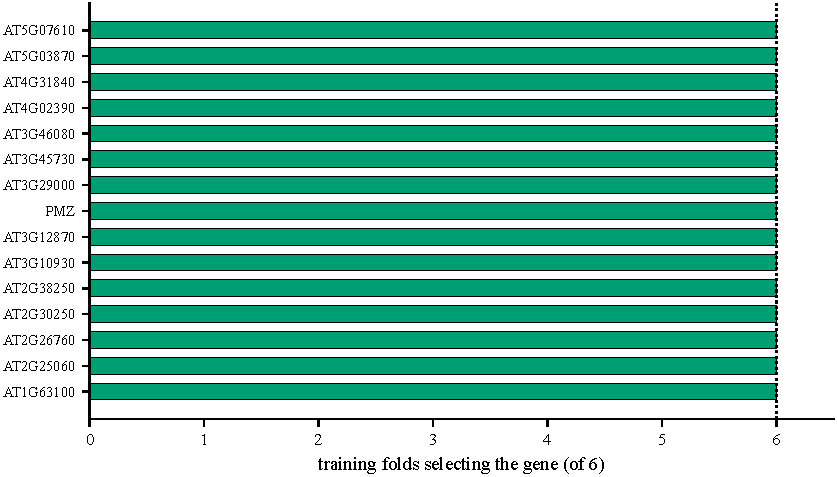
\includegraphics[width=0.78\textwidth]{fig5_stable_genes.pdf}
\caption{Genes selected most often across the six training-fold panels. A gene reaches
six only if it survives regardless of which study is held out.}
\label{fig:genes}
\end{figure*}

This concordance with the plant radiation-response
literature~\cite{culligan2006,missirian2014} makes the classifier biologically plausible.
It does not make these genes radiation biomarkers. The same DNA-damage and oxidative
programmes are induced by drought, heat, pathogens, and chemical
clastogens~\cite{missirian2014,degroote2018}, and this collection contains no
non-radiation stress controls. Specificity to radiation is untested and, on this data,
untestable.

\subsection{Exact dose remains out of reach}
\label{sec:regression}
For continuity we repeat the original regression under the identical leave-one-study-out
boundary. Gradient-boosted regression on the same matrix yields $\mathrm{MAE}=33.6$~Gy
and Spearman $\rho=0.523$ (\cref{fig:regression}). Against a dose range of $0$--$100$~Gy,
a mean absolute error of a third of the range is not a usable dosimeter, and the
predictions collapse toward the interior rather than tracking the diagonal.

\begin{figure*}[!t]
\centering
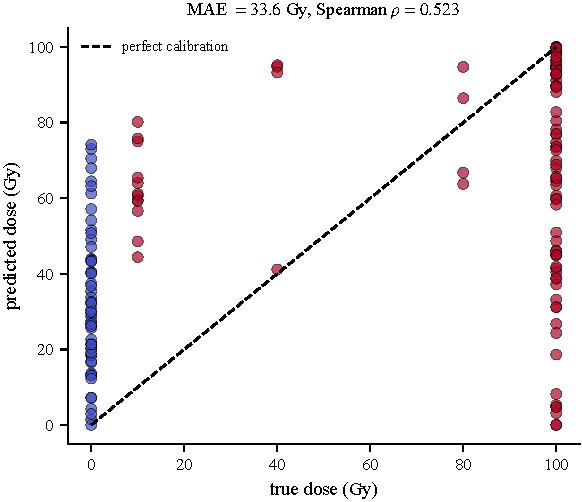
\includegraphics[width=0.52\textwidth]{fig6_dose_regression.pdf}
\caption{Secondary task: exact-dose regression under the same leave-one-study-out
protocol. Predictions cluster in the interior, the signature of a model separating two
groups rather than estimating a continuous quantity.}
\label{fig:regression}
\end{figure*}

We report this because it is the evidence for the reframing. The regression is not weak
because the model is inadequate; it is weak because $87\%$ of the design carries no
information about the interior of the dose axis.

\section{Discussion}

\subsection{Supported findings}
\begin{enumerate}
\item Changing the question improves both the science and the measured performance: the
      collection supports cross-study exposure triage and does not support exact dose
      regression.
\item The stability ensemble reaches $84.2\%$ pooled accuracy, $82.4\%$ balanced
      accuracy, $0.883$ pooled ROC-AUC, and $\mathrm{MCC}=0.656$ while holding out one
      complete study at a time.
\item Sensitivity ($89.0\%$) exceeds specificity ($75.9\%$) consistently, so the model is
      a screening instrument whose positive calls need confirmation.
\item Fold-local feature selection is essential; selecting genes before cross-validation
      would leak the held-out study.
\item With six studies, study-level bootstrap intervals span roughly $18$ percentage
      points of balanced accuracy.
\end{enumerate}

\subsection{Threats to validity}
The supplied matrix is per-study standardized, which is transductive, so the benchmark is
conditional on that representation and does not establish that a single new sample could
be normalized and scored. Six studies is a small external sample, and OSD-508's $88.9\%$
exposed fraction means one fold is close to degenerate. The selected genes are associated
with exposure in this collection but have not been tested against non-radiation
stressors. Finally, the intermediate-dose analysis rests on four samples per level and
should not be read as a dose--response result.

\subsection{The recommended next experiment}
The most valuable addition is not another model or another decimal place. It is a
genuinely untouched seventh study containing multiple doses, biological replicates, and
non-radiation stress controls, opened only after the $50/100$-gene ensemble and the
$0.5$ threshold have been frozen. That single experiment would convert an exploratory
result into a confirmatory one, and would test the specificity claim that the present
data cannot address.

\section{Model Card}
\begin{table*}[!t]
\centering
\caption{Model card~\cite{mitchell2019modelcards} for the stability ensemble.}
\label{tab:card}
\begin{tabular}{@{}p{0.26\textwidth}p{0.68\textwidth}@{}}
\toprule
Item & Statement\\
\midrule
Intended use & Research screening of exposed versus control \emph{Arabidopsis} RNA-seq samples.\\
Evaluation population & Six NASA OSDR plant studies, $158$ samples.\\
External unit & One completely held-out study.\\
Positive class & Absorbed dose greater than $0$~Gy.\\
Primary metrics & Balanced accuracy and ROC-AUC; raw accuracy is supporting.\\
Decision threshold & Fixed at $0.50$; never tuned.\\
Adaptive operations & $F$-test gene selection, scaling, and model fitting, all inside the training fold.\\
Prohibited use & Human dose estimation, individual safety decisions, or claims of causal biomarkers.\\
Known weak point & Specificity ($75.9\%$) lags sensitivity ($89.0\%$); only six external studies exist.\\
\bottomrule
\end{tabular}
\end{table*}

\section{Conclusion}
Auditing the target before modelling it changed this study's conclusion from a weak
regression to a defensible classifier. On six NASA OSDR \emph{Arabidopsis} studies, a
stability ensemble identifies radiation exposure at $84.2\%$ accuracy and $0.883$ ROC-AUC
with an entire study held out, while the exact-dose regression the design cannot support
returns $33.6$~Gy error. The governing uncertainty is the number of studies, not the
number of samples, and the study-level intervals say so plainly.

\section*{Reproducibility}
The repository contains the harmonized matrix, the sample manifest, two raw-study
examples, and the annotation tables. The figure script accompanying this manuscript
re-runs the entire leave-one-study-out benchmark, the study-level bootstrap, the gene
stability analysis, and the secondary regression from those files in under a minute on a
CPU, using scikit-learn~\cite{pedregosa2011}. Seeds, fold definitions, feature counts,
hyperparameters, target definition, and threshold are fixed in code.

\bibliographystyle{IEEEtran}
\bibliography{refs}

\end{document}
